

\tikzset{every picture/.style={line width=0.75pt}} %set default line width to 0.75pt        

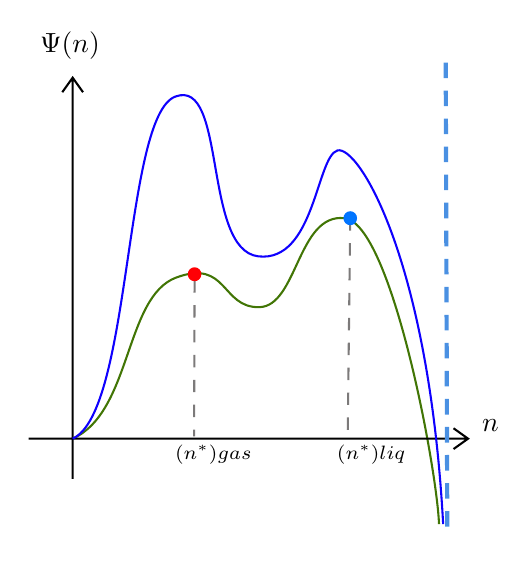
\begin{tikzpicture}[x=0.75pt,y=0.75pt,yscale=-1,xscale=1]
%uncomment if require: \path (0,300); %set diagram left start at 0, and has height of 300

%Straight Lines [id:da7707302611338531] 
\draw [color={rgb, 255:red, 124; green, 122; blue, 122 }  ,draw opacity=1 ] [dash pattern={on 4.5pt off 4.5pt}]  (235.91,136.69) -- (234.68,242.8) ;
%Straight Lines [id:da243760645874868] 
\draw [color={rgb, 255:red, 124; green, 122; blue, 122 }  ,draw opacity=1 ] [dash pattern={on 4.5pt off 4.5pt}]  (160.91,166.54) -- (160.68,241.8) ;
%Curve Lines [id:da3400867912629333] 
\draw [color={rgb, 255:red, 65; green, 117; blue, 5 }  ,draw opacity=1 ]   (102.17,242.91) .. controls (130.68,230.07) and (127.15,174.53) .. (152.03,165.3) .. controls (176.9,156.07) and (173.66,179.89) .. (192.04,179.56) .. controls (210.43,179.23) and (210.6,134.14) .. (233.14,136.69) .. controls (255.68,139.25) and (277.68,257.1) .. (278.68,284.1) ;
%Shape: Axis 2D [id:dp7159125163258058] 
\draw  (81,242.91) -- (292.68,242.91)(102.17,69) -- (102.17,262.23) (285.68,237.91) -- (292.68,242.91) -- (285.68,247.91) (97.17,76) -- (102.17,69) -- (107.17,76)  ;
%Shape: Ellipse [id:dp7614846906893419] 
\draw  [color={rgb, 255:red, 0; green, 115; blue, 255 }  ,draw opacity=1 ][fill={rgb, 255:red, 0; green, 118; blue, 255 }  ,fill opacity=1 ] (233.14,136.69) .. controls (233.14,138.27) and (234.38,139.54) .. (235.91,139.54) .. controls (237.44,139.54) and (238.68,138.27) .. (238.68,136.69) .. controls (238.68,135.12) and (237.44,133.84) .. (235.91,133.84) .. controls (234.38,133.84) and (233.14,135.12) .. (233.14,136.69) -- cycle ;
%Shape: Ellipse [id:dp14182891051606838] 
\draw  [color={rgb, 255:red, 255; green, 0; blue, 3 }  ,draw opacity=1 ][fill={rgb, 255:red, 255; green, 0; blue, 5 }  ,fill opacity=1 ] (158.14,163.69) .. controls (158.14,165.27) and (159.38,166.54) .. (160.91,166.54) .. controls (162.44,166.54) and (163.68,165.27) .. (163.68,163.69) .. controls (163.68,162.12) and (162.44,160.84) .. (160.91,160.84) .. controls (159.38,160.84) and (158.14,162.12) .. (158.14,163.69) -- cycle ;
%Straight Lines [id:da020726600111397264] 
\draw [color={rgb, 255:red, 74; green, 144; blue, 226 }  ,draw opacity=1 ][line width=1.5]  [dash pattern={on 5.63pt off 4.5pt}]  (281.91,61.69) -- (282.68,290.1) ;
%Curve Lines [id:da42260700319659494] 
\draw [color={rgb, 255:red, 15; green, 0; blue, 254 }  ,draw opacity=1 ]   (102.17,242.91) .. controls (130.68,230.07) and (126.81,87.31) .. (151.68,78.08) .. controls (176.56,68.86) and (164.68,152.08) .. (191.68,155.08) .. controls (218.68,158.08) and (219.68,107.08) .. (229.68,104.08) .. controls (239.68,101.08) and (273.68,156.08) .. (280.68,284.1) ;

% Text Node
\draw (298,232.4) node [anchor=north west][inner sep=0.75pt]    {$n$};
% Text Node
\draw (85,45.4) node [anchor=north west][inner sep=0.75pt]    {$\Psi ( n)$};
% Text Node
\draw (228,244.4) node [anchor=north west][inner sep=0.75pt]  [font=\scriptsize]  {$(n^{*})\tund{ liq}$};
% Text Node
\draw (150,244.4) node [anchor=north west][inner sep=0.75pt]  [font=\scriptsize]  {$(n^{*})\tund{ gas}$};

\end{tikzpicture}
